% arXiv manuscript source for the ADIP empirical systems study.
\documentclass[10pt]{article}

\usepackage[margin=0.78in]{geometry}
\usepackage{amsmath,amssymb}
\usepackage{booktabs}
\usepackage{graphicx}
\usepackage{microtype}
\usepackage[numbers,sort&compress]{natbib}
\usepackage{xcolor}
\usepackage{enumitem}
\usepackage{multirow}
\usepackage{placeins}
\usepackage{tikz}
\usetikzlibrary{arrows.meta,positioning,fit}
\usepackage[hidelinks]{hyperref}

% Stable manuscript terminology and claim-gated result prose.
\newcommand{\adip}{\textsc{ADIP}}
\newcommand{\vllm}{\textsc{vLLM}}
\newcommand{\gpu}{NVIDIA GeForce RTX 3060 12\,GB}
\newcommand{\model}{\texttt{Qwen2.5-1.5B-Instruct}}
\newcommand{\fixedwait}{1\,ms}
\newcommand{\adaptivecap}{20\,ms}
\newcommand{\batchcap}{8}

% Replaced by PAPER-002 after the final claim audit.
\newcommand{\HeadlineResults}{The final quantitative findings are inserted
only after all 48 declared conditions pass the terminal-state and harness audit.}
\newcommand{\PrimaryFinding}{The primary finding is pending the final
claim-to-artifact audit.}
\newcommand{\ProxyFinding}{The pass-through finding is pending the final
claim-to-artifact audit.}
\newcommand{\AdaptiveFinding}{The adaptive-policy finding is pending the final
claim-to-artifact audit.}


\title{When Batching Backfires:\\
The Hidden Cost of Adding a Gateway to Continuous LLM Serving}
\author{Wasiq\\Independent Researcher}
\date{September 2026}

\begin{document}
\maketitle

\begin{abstract}
Modern large-language-model (LLM) engines continuously batch work at token
granularity, yet production stacks often place another batching layer in an
API gateway. The interaction between these schedulers is poorly understood:
the gateway may amortize request overhead, or it may delay work that the engine
could already schedule efficiently. We present \adip{}, a compact gateway and
measurement artifact for isolating this interaction on a commodity
\gpu{}. Our central hypothesis is that, below saturation, intentional
micro-waiting is too short relative to inter-arrival time to create useful
batches; multi-request gateway batches instead emerge from backlog accumulated
while a serial gateway worker awaits the backend. We test this claim with a
predeclared, open-loop matrix comparing direct \vllm{}, gateway pass-through,
a fixed 1\,ms policy, and a frozen adaptive policy over four offered loads and
three run-level repetitions. The study records request traces, gateway queue
and backend time, batch formation, available GPU telemetry, and harness
validity.
\HeadlineResults{} The result is a reproducible account of how a second scheduler can report
larger batches while merely moving queueing in front of an engine that already
batches continuously.
\end{abstract}

\section{Introduction}
\label{sec:introduction}

An LLM request is not a single GPU operation. It begins with a parallel
prefill over the prompt and continues as an autoregressive sequence of decode
iterations. Serving engines exploit this structure by admitting and retiring
requests between iterations. Orca introduced iteration-level scheduling
\citep{yu2022orca}; \vllm{} couples continuous scheduling with PagedAttention
to reduce key--value-cache waste \citep{kwon2023pagedattention}. These engines
therefore already decide which requests share the GPU at fine granularity.

The deployment stack often adds a second scheduler. An HTTP gateway may hold
compatible requests for a few milliseconds, concatenate their prompts into one
backend call, and then split the outputs. This pattern is attractive because
batching can amortize HTTP, tokenization, and launch overhead, and it has a long
history in general prediction serving \citep{crankshaw2017clipper}. But in
front of a continuously batching LLM engine, the gateway does not create GPU
batching from nothing. It changes the time and shape in which work becomes
visible to an engine that already batches. We call this interaction
\emph{double batching}.

Double batching creates a non-obvious trade-off. Waiting can expose several
prompts in one HTTP request, but it also withholds those prompts from the
backend scheduler. A longer gateway batch can reduce per-prompt backend
overhead while worsening time to first token and head-of-line blocking. The
gateway sees only request-level completion, whereas the engine sees prefill,
decode, KV-cache pressure, and token-level progress. Optimizing the outer
scheduler without measuring the inner scheduler can therefore optimize the
wrong bottleneck.

This paper tests one falsifiable systems hypothesis:

\begin{quote}
\textbf{H:} At offered loads that direct \vllm{} can fully admit, a millisecond
gateway window is too short relative to inter-arrival time to form useful
batches. Multi-request outer batches, when they appear, are primarily backlog
coalescing caused by the gateway awaiting a backend call. Consequently, outer
batching improves latency only if the backend-time reduction from coalescing
exceeds the queueing delay and loss of scheduling freedom imposed on \vllm{}.
\end{quote}

The null hypothesis is operationally useful: fixed and adaptive gateway
batching provide no repeatable tail-latency advantage over pass-through at
matched offered load. A positive result requires a paired, run-level
improvement visible across repetitions and a latency decomposition that repays
added queueing; a negative result is evidence that the engine, not the gateway,
should own scheduling for the tested regime.

We study the question with \adip{}, an asynchronous gateway and measurement
artifact. The final matrix compares four paths---direct \vllm{}, gateway
pass-through, fixed-window batching, and a frozen adaptive policy---at
0.5, 1.0, 1.5, and 1.8 requests/s. Every condition uses identical prompts,
generation parameters, open-loop arrivals, and a single consumer-grade GPU.
Three seeds serve as the replication unit. We retain request-level latency,
queue and backend decomposition, batch identifiers and sizes, available GPU
telemetry, failures, and arrival drift.

The paper makes four contributions:

\begin{enumerate}[leftmargin=1.4em]
  \item It identifies a precise gap between engine-level continuous batching
        and request-level gateway batching, and gives a simple model separating
        \emph{window formation} from \emph{backlog formation}.
  \item It provides a tested implementation of fixed and adaptive outer
        scheduling with compatibility keys, deadline-aware closure, structured
        telemetry, and explicit cancellation and shutdown semantics.
  \item It evaluates the schedulers using predeclared open-loop arrivals and
        run-level uncertainty rather than treating requests from one run as
        independent replications.
  \item It records the complete validity trail, including interrupted and
        harness-rejected attempts, and binds final claims to machine-readable
        analysis artifacts so neutral or negative findings remain auditable.
\end{enumerate}

The scope is intentionally narrow. We do not propose a replacement for
\vllm{}, claim production-scale generality, or tune on the final matrix. The
goal is a defensible measurement study that explains a common layered-serving
decision on hardware available to an individual researcher.

\section{Background and Related Work}
\label{sec:background}

\subsection{Why LLM batching is different}

Conventional request-level batching waits for several inputs, executes one
tensor program, and releases the batch when all outputs are ready. Generative
inference has two asymmetric phases. Prefill processes many prompt tokens in
parallel and is typically compute intensive; decode processes one new token per
active sequence and is often memory-bandwidth limited. Request lengths vary,
so static batches suffer from head-of-line blocking. Orca's iteration-level
scheduler allows the active set to change between decode iterations
\citep{yu2022orca}. PagedAttention reduces fragmentation in the dynamically
growing KV cache and enables \vllm{} to sustain larger active sets
\citep{kwon2023pagedattention}.

Recent systems optimize this inner schedule. Sarathi-Serve uses chunked
prefills and stall-free schedules to reduce prefill--decode interference
\citep{agrawal2024sarathiserve}. DeepSpeed-FastGen's Dynamic SplitFuse also
decomposes prompts and generations to balance throughput and latency
\citep{holmes2024fastgen}. DistServe separates prefill and decode resources to
optimize goodput under distinct latency objectives \citep{zhong2024distserve}.
These systems have detailed visibility into token-level execution. \adip{}
does not: it treats \vllm{} as a black-box HTTP backend and asks what an outer
layer can accomplish with request-level signals alone.

\subsection{Layered prediction serving}

Clipper demonstrated that a serving layer can batch calls to otherwise
unmodified ML frameworks and adapt batch size to a latency objective
\citep{crankshaw2017clipper}. That result motivates gateway batching, but the
backend models in classical prediction serving usually execute a bounded
forward pass. An LLM backend is itself a stateful scheduler. Outer batching
therefore changes both transport granularity and the arrival process observed
by the inner scheduler.

The workload also matters. BurstGPT shows that real LLM services exhibit
time-varying concurrency, response lengths, and failures, and warns that
scheduling conclusions may not generalize across traces
\citep{wang2024burstgpt}. Our primary experiment deliberately uses a
deterministic constant-rate workload. This sacrifices trace realism to isolate
the mechanism; burst sensitivity is left as future validation rather than
being implied by the constant-rate result.

\subsection{Window formation versus backlog formation}
\label{sec:mechanism-model}

Let $\lambda$ be the request arrival rate and $w$ the gateway's intentional
wait window. Under a Poisson approximation, useful for intuition even though
our primary arrivals are deterministic,
\begin{equation}
  \mathbb{E}[N_w] = \lambda w, \qquad
  P(N_w \ge 1) = 1-e^{-\lambda w},
  \label{eq:window}
\end{equation}
where $N_w$ is the number of companion arrivals during the window. At the
largest tested rate, 1.8 requests/s, a 1\,ms window yields
$\mathbb{E}[N_w]=0.0018$ and $P(N_w\ge1)\approx0.18\%$. Even a 20\,ms cap
yields only 0.036 expected companions and a 3.54\% probability. Intentional
micro-waiting alone should therefore produce almost exclusively singleton
batches in this regime.

Now let $S$ be the time for which a serial gateway worker awaits one backend
call. Requests continue to arrive during that interval, creating approximately
$\lambda S$ queued companions. When the worker returns and drains the ingress
queue, it can dispatch a multi-request backend call even if $w$ is nearly zero.
This \emph{backlog coalescing} is qualitatively different from
Eq.~\ref{eq:window}: its control variable is service occupancy, not the
micro-wait. It also exposes the cost of a serial outer scheduler. A request
that arrives behind an in-flight call cannot reach \vllm{} until the outer
worker returns, even though \vllm{} could otherwise admit it into continuous
batching.

Our evaluation tests which mechanism dominates by jointly examining observed
batch size, gateway queue time, backend time, achieved throughput, and tail
latency. This mechanism-level accounting is the paper's main distinction from
a benchmark that merely ranks configurations.

\section{Research Questions and Methodology}
\label{sec:methodology}

\subsection{Research questions}

We organize the evaluation around three questions.

\begin{description}[leftmargin=3.2em,style=nextline]
  \item[RQ1: Layering cost.] What latency and utilization change is introduced
        by a pass-through gateway relative to direct \vllm{}?
  \item[RQ2: Outer batching.] At matched offered load, does fixed gateway
        batching improve throughput or latency after accounting for queue time
        and the backend's own continuous batching?
  \item[RQ3: Adaptation.] Does a frozen low-load bypass policy avoid harmful
        waiting while preserving useful backlog coalescing?
\end{description}

For RQ2 and RQ3, the confirmatory comparison is paired by repetition seed.
The null is zero mean paired difference. We report effect direction and 95\%
Student-$t$ intervals over three run-level differences; we do not label a
difference statistically significant from request counts within a run.

\subsection{Testbed}

All measurements run locally in WSL2 Ubuntu on a Windows host with an
\gpu{}. The backend is \vllm{} 0.29.0 in eager mode with float16 weights,
maximum model length 2,048, GPU-memory utilization 0.85, and at most eight
sequences. The model is \model{} at immutable revision
\texttt{989aa7980e4cf806f80c7fef2b1adb7bc71aa306}
\citep{qwen2025technical}. Generation is deterministic
($T=0$) with at most 64 output tokens. Direct traffic targets port 8001;
gateway modes target \adip{} on port 8000, which forwards to the same backend.

\begin{table}[t]
  \centering
  \small
  \caption{Frozen primary experiment. Every cell has three run-level
  repetitions.}
  \label{tab:experiment}
  \begin{tabular}{ll}
    \toprule
    Factor & Value \\
    \midrule
    GPU & NVIDIA RTX 3060, 12\,GB \\
    Model & Qwen2.5-1.5B-Instruct, float16 \\
    Backend & vLLM 0.29.0, eager execution \\
    Modes & direct, pass-through, fixed, adaptive \\
    Offered rates & 0.5, 1.0, 1.5, 1.8 requests/s \\
    Prompt bucket & 8--128 tokenizer-derived input tokens \\
    Output cap & 64 tokens \\
    Warmup & 50 sequential requests per condition \\
    Measurement & 120 seconds, open loop \\
    Repetitions & seeds 1729, 2718, 3141 \\
    Fixed policy & max batch 8, max wait 1\,ms \\
    Adaptive policy & max batch 8, max wait 20\,ms \\
    \bottomrule
  \end{tabular}
\end{table}

\subsection{Workload and controls}

The workload is synthetic and length controlled, not a production trace. Four
project-authored seed passages are expanded deterministically until they fall
inside the 8--128 token bucket under the exact model tokenizer. All requests
use the same model, output cap, and temperature, making them compatible for
gateway batching. The benchmark generates the complete constant-rate arrival
schedule before execution. Each request sleeps until an absolute target time;
later requests do not wait for earlier completions. This open-loop design
avoids coordinated omission when the system slows down.

Fifty warmup requests precede each measured interval. Warmups are excluded
from every aggregate. A five-second cooldown separates conditions. The final
matrix contains $4\times4\times3=48$ conditions and 5,760 seconds of measured
traffic, excluding warmup and cooldown. The fixed 1\,ms comparator and adaptive
parameters were frozen from calibration and pilot data before the final matrix.
The runner executes the declared order by mode (direct, pass-through, fixed,
adaptive), then repetition, then increasing rate. This deterministic order
makes interruption recovery auditable but does not balance slow temporal or
thermal drift. Seed pairing controls workload construction, not wall-clock
position; we treat the lack of randomized interleaving as a validity
limitation rather than implying otherwise.

\subsection{Validity gate and failure accounting}

Host scheduling can invalidate an open-loop experiment even when the server
returns success. We therefore record target and actual arrival time for every
request. A condition is marked \texttt{invalid\_harness} when more than 1\%
of measured requests arrive over 50\,ms late. The raw records remain stored,
but the condition is excluded from performance claims. Ordinary incomplete
directories are rejected by the resume logic rather than appended to. Request
failures remain in the denominator and are never converted to zero latency.

\subsection{Metrics and uncertainty}

The request is the latency observation unit; the run is the replication unit.
For each run we compute achieved requests/s, output tokens/s, success and
failure counts, p50/p95/p99 end-to-end latency, mean and p95 gateway queue time,
mean backend time, mean batch size, GPU utilization, peak VRAM, power, and p95
arrival drift. We then average the three run-level values for each condition
and report a two-sided 95\% Student-$t$ interval. With only three repetitions,
these intervals are necessarily wide; figures show each run point to prevent
the mean from hiding instability.

Each request record carries its outer batch ID and reported batch size. A
request-wise average of that field is size biased: a group of four contributes
four observations while a singleton contributes one. For mechanism claims we
therefore group records by batch ID and report the call-weighted mean number of
prompts per backend HTTP call. The raw request-weighted mean remains in each
run summary for auditability but is not labeled as a call-level average. The
same unique-call grouping yields $\bar S_{\mathrm{call}}$ for
Eq.~\ref{eq:occupancy-prediction}; the analyzer reports measured group size,
predicted group size, and their ratio for every fixed and adaptive run.

The primary effects are paired by rate and seed:
\begin{align}
  \Delta_{\mathrm{proxy}} &= M_{\mathrm{pass}}-M_{\mathrm{direct}},\\
  \Delta_{\mathrm{fixed}} &= M_{\mathrm{fixed}}-M_{\mathrm{pass}},\\
  \Delta_{\mathrm{adaptive}} &= M_{\mathrm{adaptive}}-M_{\mathrm{fixed}},
\end{align}
for metric $M$. Absolute and relative deltas are both retained. We interpret
throughput separately from goodput and offered load separately from achieved
load.

\section{ADIP Design}
\label{sec:design}

\subsection{Two scheduling layers}

Figure~\ref{fig:architecture} shows the paths under comparison. Direct mode
sends one OpenAI-compatible completion per client request. Pass-through adds
HTTP translation and telemetry but calls the backend once per request. Fixed
and adaptive modes place requests in compatibility-keyed queues and send one
backend prompt list per outer batch. In every mode, \vllm{} retains control of
its token-level continuous scheduler.

\begin{figure}[t]
  \centering
  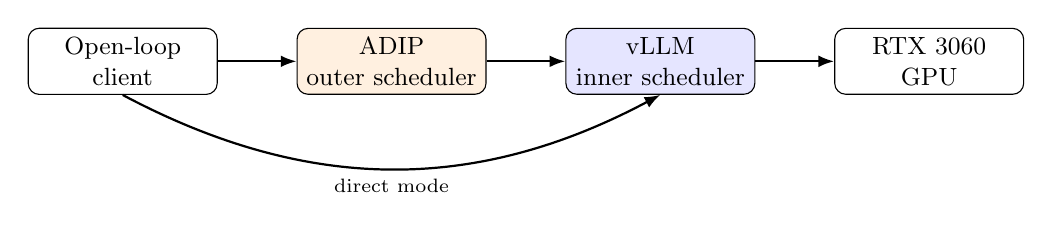
\begin{tikzpicture}[
    node distance=10mm,
    box/.style={draw,rounded corners,align=center,minimum height=8mm,minimum width=24mm,font=\small},
    sched/.style={box,fill=orange!12},
    engine/.style={box,fill=blue!10},
    arrow/.style={-{Latex[length=2mm]},thick}
  ]
    \node[box] (client) {Open-loop\\client};
    \node[sched,right=of client] (gateway) {ADIP\\outer scheduler};
    \node[engine,right=of gateway] (vllm) {vLLM\\inner scheduler};
    \node[box,right=of vllm] (gpu) {RTX 3060\\GPU};
    \draw[arrow] (client) -- (gateway);
    \draw[arrow] (gateway) -- (vllm);
    \draw[arrow] (vllm) -- (gpu);
    \draw[arrow,bend right=28] (client.south) to node[below,font=\scriptsize]{direct mode} (vllm.south);
  \end{tikzpicture}
  \caption{The experimental boundary. Gateway batching controls when and in
  what HTTP grouping prompts become visible; \vllm{} independently controls
  token-level GPU scheduling.}
  \label{fig:architecture}
\end{figure}

\subsection{Compatibility and queue discipline}

A batch key consists of model identifier, output-token cap, and temperature.
Only equal keys share a backend request. The ingress queue is bounded; a full
queue rejects before creating unresolved work. One coordinator drains ingress
into per-key FIFO queues, selects the oldest compatible queue, obtains a pure
policy decision, and awaits one backend batch. This simple coordinator makes
the mechanism measurable, but it is intentionally serial: arrivals during a
backend call accumulate until that call returns. Section~\ref{sec:mechanism-model}
predicts that this occupancy-driven backlog can dominate the nominal
micro-wait.

\subsection{Fixed batch closure}

For the oldest compatible queue, the fixed policy dispatches when (i) the batch
reaches eight requests, (ii) the oldest request reaches the 1\,ms window, or
(iii) further waiting would consume estimated service slack before the earliest
soft deadline. Otherwise it waits only for the remaining window. Policy code
does not perform I/O or sleep; the coordinator owns timing and queue mutation.

\subsection{Adaptive closure}

The adaptive policy was frozen before final evaluation. It maintains
exponentially weighted moving averages of compatible arrival rate $\hat\lambda$
and backend time $\hat S$ with smoothing factor 0.2. For remaining window
$w_r$, it computes expected companions $\hat\lambda w_r$. If this value is
below 1.0, it dispatches immediately. Otherwise it waits for the minimum of
the remaining 20\,ms cap, estimated time to fill the batch,
\begin{equation}
  t_{\mathrm{fill}}=
  \frac{B_{\max}-B_{\mathrm{queue}}}{\hat\lambda},
\end{equation}
and positive deadline slack after reserving $\hat S$. Full queues, expired
windows, and exhausted slack dispatch immediately. Importantly, low-load
bypass does not split requests already accumulated during an in-flight backend
call; it closes the existing backlog without adding intentional wait.

\subsection{Instrumentation and failure semantics}

Every accepted request receives a UUID and optional experiment identifier.
Structured events record enqueue, policy reason, batch dispatch, backend
completion, and request completion without prompt text or credentials. The
response carries batch ID, batch size, queue time, backend time, total gateway
time, and deadline outcome. Backend failures resolve every future in the
affected batch. Cancellation and shutdown settle queued and in-flight futures
exactly once, preventing a successful test run from hiding leaked asynchronous
work.

The benchmark writes request JSONL as each request completes, while a separate
sampler records GPU utilization, VRAM, power, and temperature through
\texttt{nvidia-smi}. A manifest created before traffic binds the run to the
Git commit, model revision, mode, rate, seed, and frozen parameters. Atomic
summary writes occur only after traffic and validity checks complete.

\section{Evaluation}
\label{sec:evaluation}

The final evaluation is populated by the claim-audited output of
\texttt{python -m bench.analyze\_final}. The script refuses to run until all
48 declared conditions are terminal and keeps any harness-invalid condition in
explicit exclusion accounting. This section is organized by research question
rather than by implementation component.

\subsection{RQ1: What does the pass-through layer cost?}

\ProxyFinding

\IfFileExists{figures/primary_overview.pdf}{
\begin{figure*}[t]
  \centering
  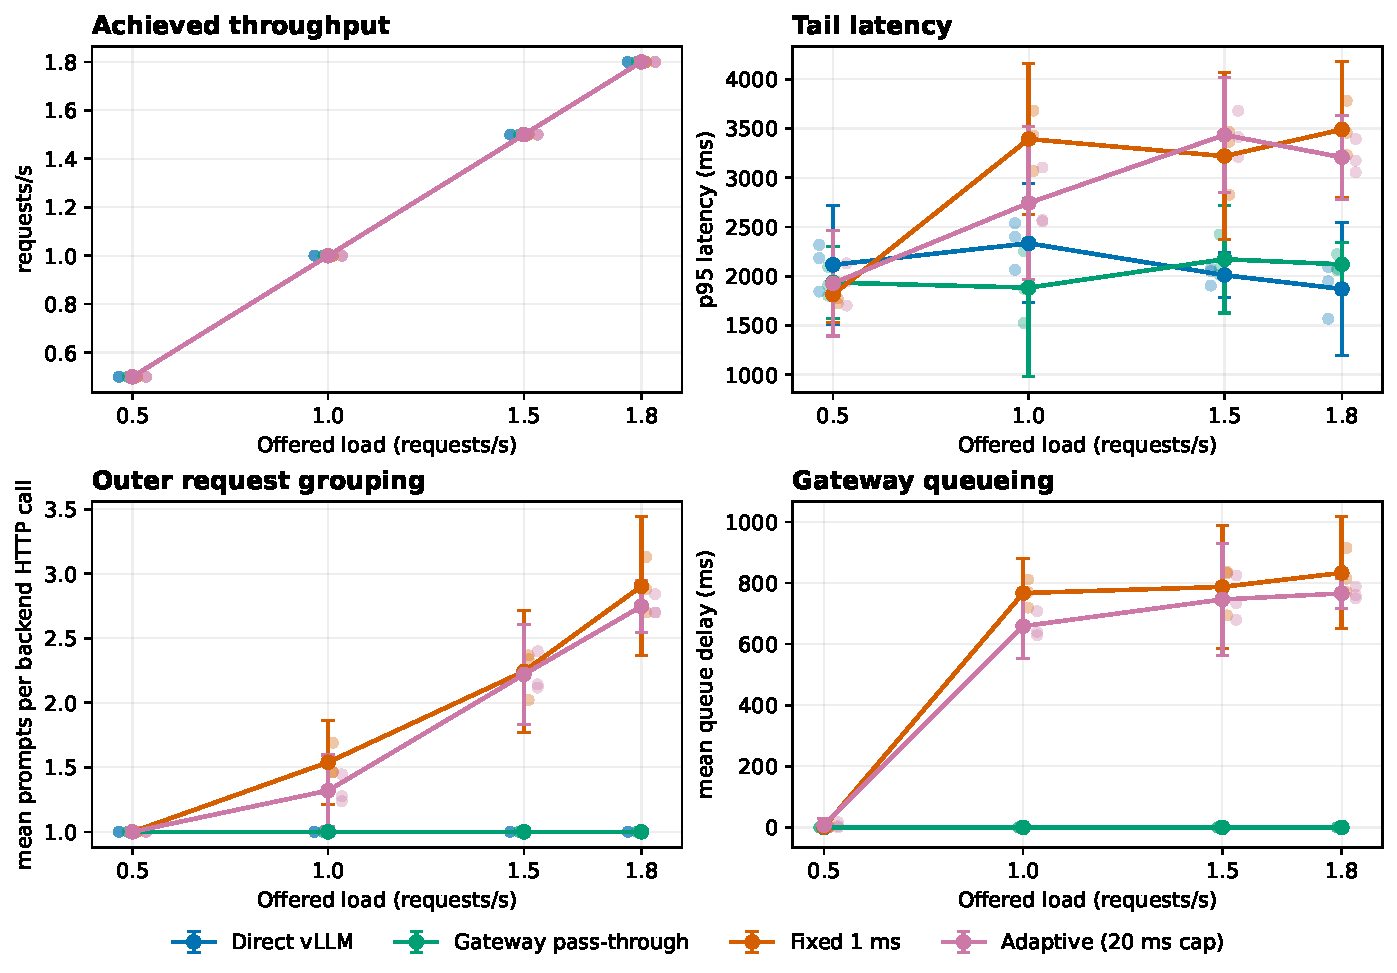
\includegraphics[width=0.96\textwidth]{figures/primary_overview.pdf}
  \caption{Primary matrix on \model{} and one \gpu{}. Lines show means across
  three run-level repetitions; error bars are two-sided 95\% Student-$t$
  intervals; translucent points are individual repetitions. Offered load is
  fixed by the open-loop schedule. Outer request grouping is call-weighted
  prompts per backend HTTP call, not \vllm{}'s token-level active set.}
  \label{fig:overview}
\end{figure*}
}{}

\subsection{RQ2: Does fixed outer batching help?}

\PrimaryFinding

\IfFileExists{tables/primary_results.tex}{
\begin{table*}[t]
  \centering
  \small
  \caption{All primary conditions. Values are run-level mean $\pm$ 95\%
  Student-$t$ half-width over three repetitions. Throughput is achieved
  successful requests/s.}
  \label{tab:primary}
  \resizebox{\textwidth}{!}{% Generated by python -m bench.analyze_final; do not edit by hand.
\begin{tabular}{llrrrr}
\toprule
Mode & Rate & Throughput & p95 latency & Outer group & Queue delay \\
 & (req/s) & (req/s) & (ms) & (requests) & (ms) \\
\midrule
Direct vLLM & 0.5 & 0.50 $\pm$ 0.00 & 2115 $\pm$ 607 & 1.00 $\pm$ 0.00 & -- \\
Direct vLLM & 1.0 & 1.00 $\pm$ 0.00 & 2334 $\pm$ 605 & 1.00 $\pm$ 0.00 & -- \\
Direct vLLM & 1.5 & 1.50 $\pm$ 0.00 & 2010 $\pm$ 229 & 1.00 $\pm$ 0.00 & -- \\
Direct vLLM & 1.8 & 1.80 $\pm$ 0.00 & 1870 $\pm$ 674 & 1.00 $\pm$ 0.00 & -- \\
\addlinespace
Gateway pass-through & 0.5 & 0.50 $\pm$ 0.00 & 1935 $\pm$ 367 & 1.00 $\pm$ 0.00 & 0 $\pm$ 0 \\
Gateway pass-through & 1.0 & 1.00 $\pm$ 0.00 & 1884 $\pm$ 906 & 1.00 $\pm$ 0.00 & 0 $\pm$ 0 \\
Gateway pass-through & 1.5 & 1.50 $\pm$ 0.00 & 2172 $\pm$ 546 & 1.00 $\pm$ 0.00 & 0 $\pm$ 0 \\
Gateway pass-through & 1.8 & 1.80 $\pm$ 0.00 & 2120 $\pm$ 223 & 1.00 $\pm$ 0.00 & 0 $\pm$ 0 \\
\addlinespace
Fixed 1 ms & 0.5 & 0.50 $\pm$ 0.00 & 1812 $\pm$ 280 & 1.00 $\pm$ 0.00 & 2 $\pm$ 1 \\
Fixed 1 ms & 1.0 & 1.00 $\pm$ 0.00 & 3393 $\pm$ 763 & 1.54 $\pm$ 0.33 & 767 $\pm$ 114 \\
Fixed 1 ms & 1.5 & 1.50 $\pm$ 0.00 & 3220 $\pm$ 850 & 2.24 $\pm$ 0.48 & 788 $\pm$ 201 \\
Fixed 1 ms & 1.8 & 1.80 $\pm$ 0.00 & 3490 $\pm$ 687 & 2.90 $\pm$ 0.54 & 833 $\pm$ 183 \\
\addlinespace
Adaptive (20 ms cap) & 0.5 & 0.50 $\pm$ 0.00 & 1927 $\pm$ 535 & 1.00 $\pm$ 0.00 & 7 $\pm$ 21 \\
Adaptive (20 ms cap) & 1.0 & 1.00 $\pm$ 0.00 & 2744 $\pm$ 777 & 1.32 $\pm$ 0.28 & 659 $\pm$ 106 \\
Adaptive (20 ms cap) & 1.5 & 1.50 $\pm$ 0.00 & 3435 $\pm$ 583 & 2.22 $\pm$ 0.39 & 746 $\pm$ 182 \\
Adaptive (20 ms cap) & 1.8 & 1.80 $\pm$ 0.00 & 3208 $\pm$ 426 & 2.75 $\pm$ 0.20 & 766 $\pm$ 50 \\
\bottomrule
\end{tabular}
}
\end{table*}
}{}

\IfFileExists{figures/mechanism_effects.pdf}{
\begin{figure*}[t]
  \centering
  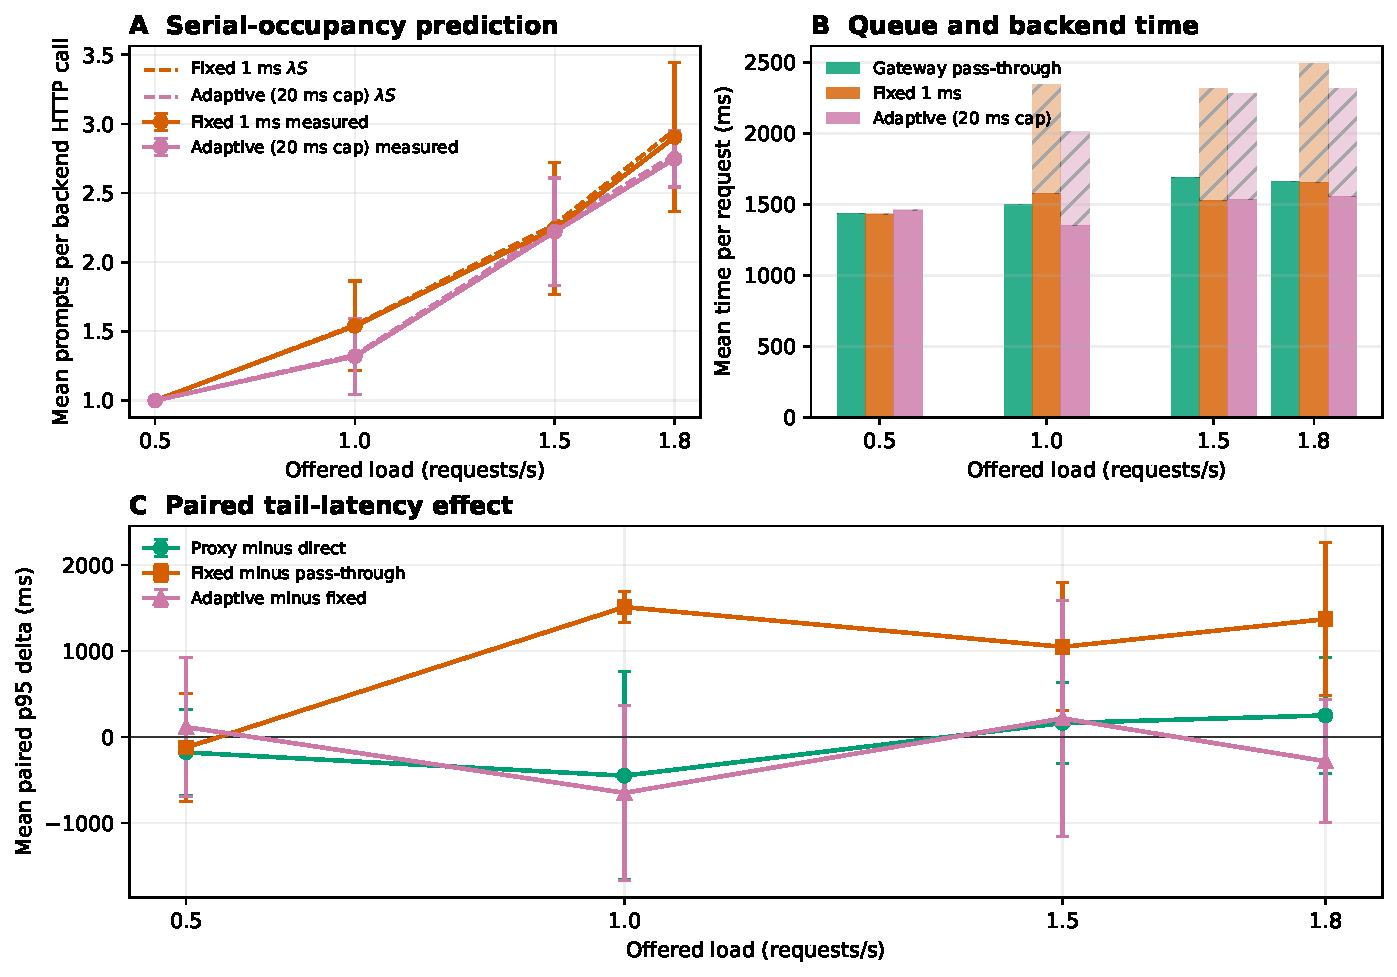
\includegraphics[width=0.96\textwidth]{figures/mechanism_effects.pdf}
  \caption{Mechanism accounting for \model{} on one \gpu{}. Panel A compares
  measured call-weighted outer grouping with the serial-occupancy prediction
  $\max(1,\lambda\bar S_{\mathrm{call}})$. Panel B separates gateway queue
  and backend time; hatching denotes queue time stacked above backend time.
  Panel C shows paired p95-latency effects by repetition seed. Error bars are
  two-sided 95\% Student-$t$ intervals over three run-level values or paired
  differences.}
  \label{fig:mechanism}
\end{figure*}
}{}

\subsection{RQ3: Does the frozen adaptive policy help?}

\AdaptiveFinding

\IfFileExists{tables/paired_effects.tex}{
\begin{table}[t]
  \centering
  \scriptsize
  \caption{Paired p95-latency effects. Positive values mean the treatment is
  slower than its comparator. Values are mean $\pm$ 95\% Student-$t$
  half-width across shared repetition seeds.}
  \label{tab:effects}
  \resizebox{\columnwidth}{!}{% Generated by python -m bench.analyze_final; do not edit by hand.
\begin{tabular}{lrrr}
\toprule
Comparison & Rate & p95 delta (ms) & Relative delta (\%) \\
\midrule
Proxy minus direct & 0.5 & -180 $\pm$ 496 & -8.0 $\pm$ 20.9 \\
Proxy minus direct & 1.0 & -451 $\pm$ 1212 & -18.4 $\pm$ 46.4 \\
Proxy minus direct & 1.5 & 162 $\pm$ 472 & 8.0 $\pm$ 22.9 \\
Proxy minus direct & 1.8 & 251 $\pm$ 675 & 15.0 $\pm$ 42.3 \\
Fixed minus pass-through & 0.5 & -123 $\pm$ 631 & -5.7 $\pm$ 31.6 \\
Fixed minus pass-through & 1.0 & 1510 $\pm$ 180 & 82.6 $\pm$ 47.3 \\
Fixed minus pass-through & 1.5 & 1047 $\pm$ 744 & 48.7 $\pm$ 40.2 \\
Fixed minus pass-through & 1.8 & 1370 $\pm$ 886 & 65.1 $\pm$ 47.6 \\
Adaptive minus fixed & 0.5 & 115 $\pm$ 811 & 7.1 $\pm$ 45.0 \\
Adaptive minus fixed & 1.0 & -650 $\pm$ 1019 & -18.8 $\pm$ 26.1 \\
Adaptive minus fixed & 1.5 & 216 $\pm$ 1373 & 8.0 $\pm$ 47.6 \\
Adaptive minus fixed & 1.8 & -282 $\pm$ 713 & -7.8 $\pm$ 18.4 \\
\bottomrule
\end{tabular}
}
\end{table}
}{}

\subsection{Validity and negative-result accounting}

The final paper reports the exact number of complete, harness-invalid, failed,
and interrupted runs. Interrupted attempts are operational history, not
samples. Any harness-invalid terminal condition remains visible with its
predeclared reason but contributes to no performance mean. If fewer than three
valid repetitions remain for a condition, we report the reduced $n$ and avoid
a confirmatory claim for that comparison.

\section{Discussion and Limitations}
\label{sec:discussion}

\subsection{Interpreting a second scheduler}

The crucial distinction is between forming a batch by waiting and forming one
because the outer worker was already busy. The former can be tuned with a
micro-window; the latter is a consequence of serial service occupancy. If
observed batch size rises while intentional companion probability remains near
zero, backlog coalescing is the parsimonious explanation. Whether that is
beneficial depends on the full latency decomposition. Lower backend time does
not imply lower end-to-end latency when the same policy increases queue time or
withholds prompts from continuous batching.

This distinction also changes how an adaptive policy should be judged. A
low-load bypass can correctly decide never to wait and still emit multi-request
batches after a backend call. Calling such behavior ``adaptive waiting'' would
be misleading; it is adaptive \emph{closure} of backlog. A future gateway that
wants to coordinate rather than compete with \vllm{} may need multiple
concurrent backend calls, token-level feedback, or an engine-native scheduling
interface. Those are different designs from a black-box HTTP batcher.

\subsection{Practical decision rule}

For a gateway operator, the first question should be whether direct \vllm{}
already achieves the offered load within the latency objective. If it does,
outer batching must demonstrate an end-to-end improvement, not merely a larger
batch size. At low $\lambda w$, a fixed window has little opportunity to find
companions and should default to pass-through. At high $\lambda S$, a serial
gateway will coalesce backlog automatically, but operators should inspect queue
growth and tail latency before treating this as a throughput optimization.
The safest default is therefore engine-owned batching with gateway
instrumentation; enable outer coalescing only when paired measurements show
that reduced backend cost exceeds added queueing for the target workload.

\subsection{Threats to validity}

\textbf{Hardware and runtime.} The study uses one consumer GPU under WSL2 and
the Windows display-driver model. Absolute latency, host scheduling, power,
and thermal behavior may differ on native Linux or datacenter GPUs. We treat
arrival drift as a validity variable precisely because the host is part of the
measured system.

\textbf{Model and workload.} \model{} is small enough to run reproducibly on
12\,GB VRAM. Larger models, long contexts, quantization, tensor parallelism,
and speculative decoding can change service time and the balance between
prefill and decode. The primary workload uses short, synthetic prompts,
constant arrivals, and a 64-token output cap. Real traces are bursty and
heterogeneous \citep{wang2024burstgpt}; our result should not be generalized to
them without the planned sensitivity study.

\textbf{Load range.} The evaluated rates are calibration-derived points up to
1.8 requests/s. They test a regime in which direct service accepts all offered
traffic, not maximum sustainable saturation. This is deliberate for testing
the hypothesis, but it does not establish the gateway's overload capacity.

\textbf{Statistics.} Three repetitions support paired mechanism evidence but
only coarse uncertainty estimates. Student-$t$ intervals with two degrees of
freedom are sensitive to any outlying run. We therefore show individual run
points and avoid significance language unsupported by the interval.

\textbf{Implementation boundary.} \adip{} uses one coordinator that awaits a
backend batch. The measured backlog mechanism is specific to this transparent,
serial outer architecture. A pipelined or concurrent gateway could expose
arrivals to \vllm{} sooner, while an engine-integrated policy could access
token-level state. The paper characterizes a common and intentionally simple
design, not every possible gateway.

\textbf{Metric boundary.} End-to-end request latency is the principal outcome.
The completions API does not expose token streaming in this experiment, so we
do not separately report time to first token and time per output token. A
system optimized for interactive streaming may require those objectives.

\subsection{Reproducibility as a result}

The artifact separates exploratory pilot evidence from final claims, freezes
policy parameters before the primary matrix, records every exclusion, and
computes uncertainty across runs. This discipline matters for small-system
research: a negative result with a complete causal trail is more informative
than a large percentage derived from one favorable run. The code, configs,
tests, raw-schema definitions, and analysis scripts are intended to make every
number in the final paper traceable to named run IDs.

\section{Conclusion}
\label{sec:conclusion}

Gateway micro-batching in front of a continuously batching LLM engine is not a
free second optimization. It is a second scheduler with less information and
its own queue. This paper separates two mechanisms that are easy to conflate:
companions found during an intentional micro-window and backlog accumulated
while a serial outer worker awaits the backend. \adip{} turns that distinction
into a falsifiable, request-level experiment on commodity hardware.

\PrimaryFinding\ \AdaptiveFinding
Within the tested scope, the practical conclusion follows the full
throughput--latency decomposition, not batch size alone. The artifact and
methodology make that conclusion auditable and provide a base for bursty,
heterogeneous, and larger-model validation without changing the frozen primary
hypothesis.


\bibliographystyle{plainnat}
\bibliography{references}

\appendix
\section{Reproduction checklist}
\label{app:reproduction}
The artifact pins the model revision, Python and vLLM environments, generation
parameters, workload seeds, and experiment configuration. Each run directory
contains a manifest, append-only request records, GPU samples, and a generated
summary. The analysis validates all declared conditions before producing
figures or tables. Raw invalid or interrupted attempts remain in dated archive
directories and are never pooled with final runs. The repository includes the
exact LuaLaTeX/BibTeX build sequence and a progress ledger that records each
execution and recovery decision.

\end{document}
